% Created 2016-08-17 Wed 14:38
\documentclass[tikz]{standalone}

\usepackage[utf8]{inputenc}
\usepackage[T1]{fontenc}
\usepackage{helvet}
\usepackage{../../templates/msc}

\renewcommand{\familydefault}{\sfdefault}

\tikzset{
every picture/.style={
line width=1pt
}}

\usepackage{tikz}
\author{Holger Karl}
\date{\today}
\title{}

\usetikzlibrary{positioning, calc}

\usetikzlibrary{intersections}


\newcommand{\timeline}[1]{
  \draw [-> ] (0,0) --  (#1,0) node [below, auto] {time} ;
  \draw [-> ] (0,0) -- (0, 4) node [left=0.75cm, auto, rotate=90]  {processes};
  
  \foreach \i in {1,2,3} {
    \draw [thin , name path=p\i] (0,\i) --  (#1,\i);
    \node [left] at (0, \i) {$P_\i$};
  }
}

\newcommand{\basicpic}{
  \timeline{8}

  \foreach \x/\y/\l [count=\i]in { 1/2/1, 3/3/2, 5/1/3, 7/2/4} {
    \node [circle, draw, fill=white] (\i) at (\x, \y) {\l};
  }
  \draw [->] (1) to node [auto, near start] {$m_1$} (2); 
  \draw [->] (3) to node [auto, near end, auto ] {$m_3$} (4); 
}

\newcommand{\intersectcut}{
    \foreach \i in {1,2,3} {
      \path [name intersections={of=cut and p\i, by={tmp}}];
      \node [circle, draw, fill=red!10, inner sep=1pt ] at (tmp) {\small $S_\i$};
    }
  }

\begin{document}


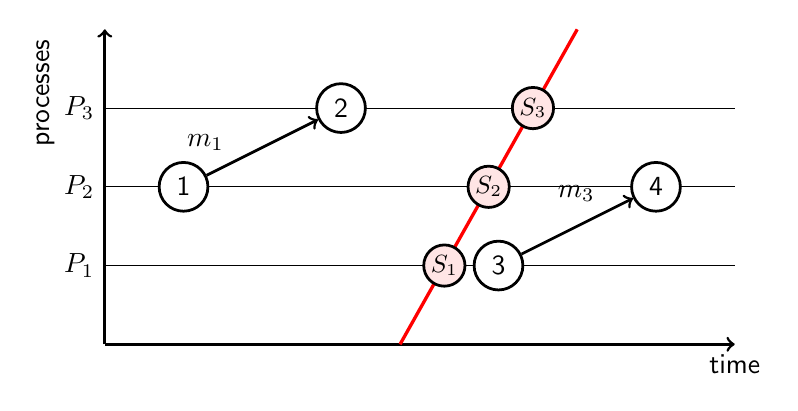
\begin{tikzpicture}

  % events 
  \basicpic 
  
  \draw [very thick, red, name path=cut] (3.75, 0) -- (6,4);

  \intersectcut

\end{tikzpicture}


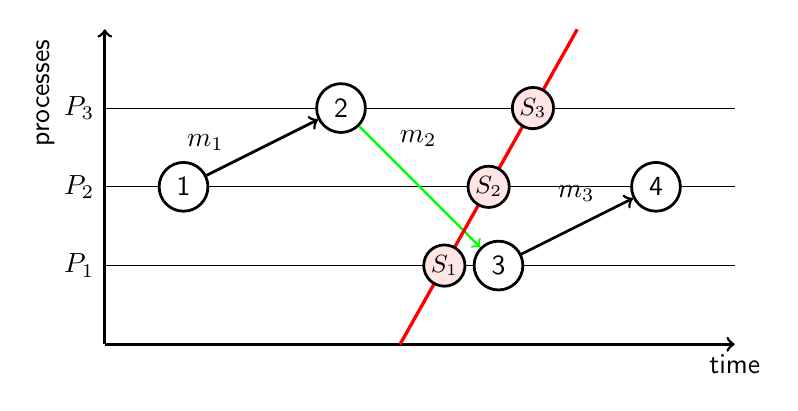
\begin{tikzpicture}
  \basicpic 

  \draw [->, thick, green, near start] (2) to node  [black, auto] {$m_2$} (3) ;
  
  \draw [very thick, red, name path=cut] (3.75, 0) -- (6,4);
  \intersectcut

\end{tikzpicture}


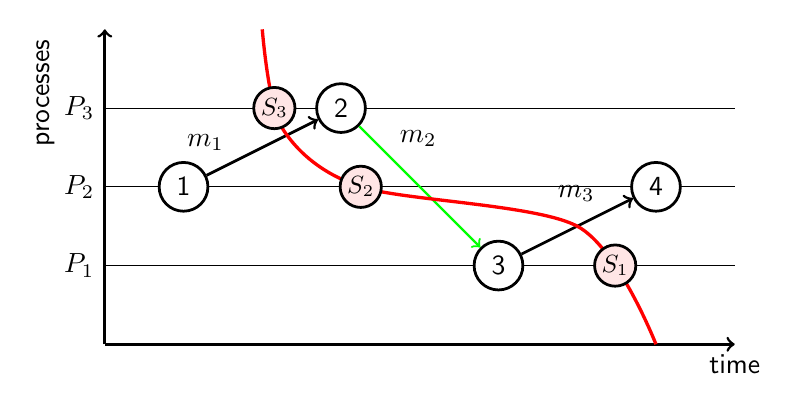
\begin{tikzpicture}
  \basicpic 

  \draw  [->, thick, green, , near start, name path=mess] (2)  to node [black, auto]{$m_2$} (3) ; 
  
  % \draw [very thick, red] (2, 4) -- (2.25, 2.75) -- (3.5, 2) -- (6, 1.5)  -- (7,0);
  \draw [very thick, red, name path=cut]  plot [smooth] coordinates
  {(2, 4)  (2.25, 2.75)  (3.25, 2)  (6, 1.5)   (7,0)};

  % \path [name intersections={of=mess and cut, by={XX}}];
  % \node [above] at (XX) {??};
  
  \intersectcut


\end{tikzpicture}


\end{document}

